\usetikzlibrary{arrows}
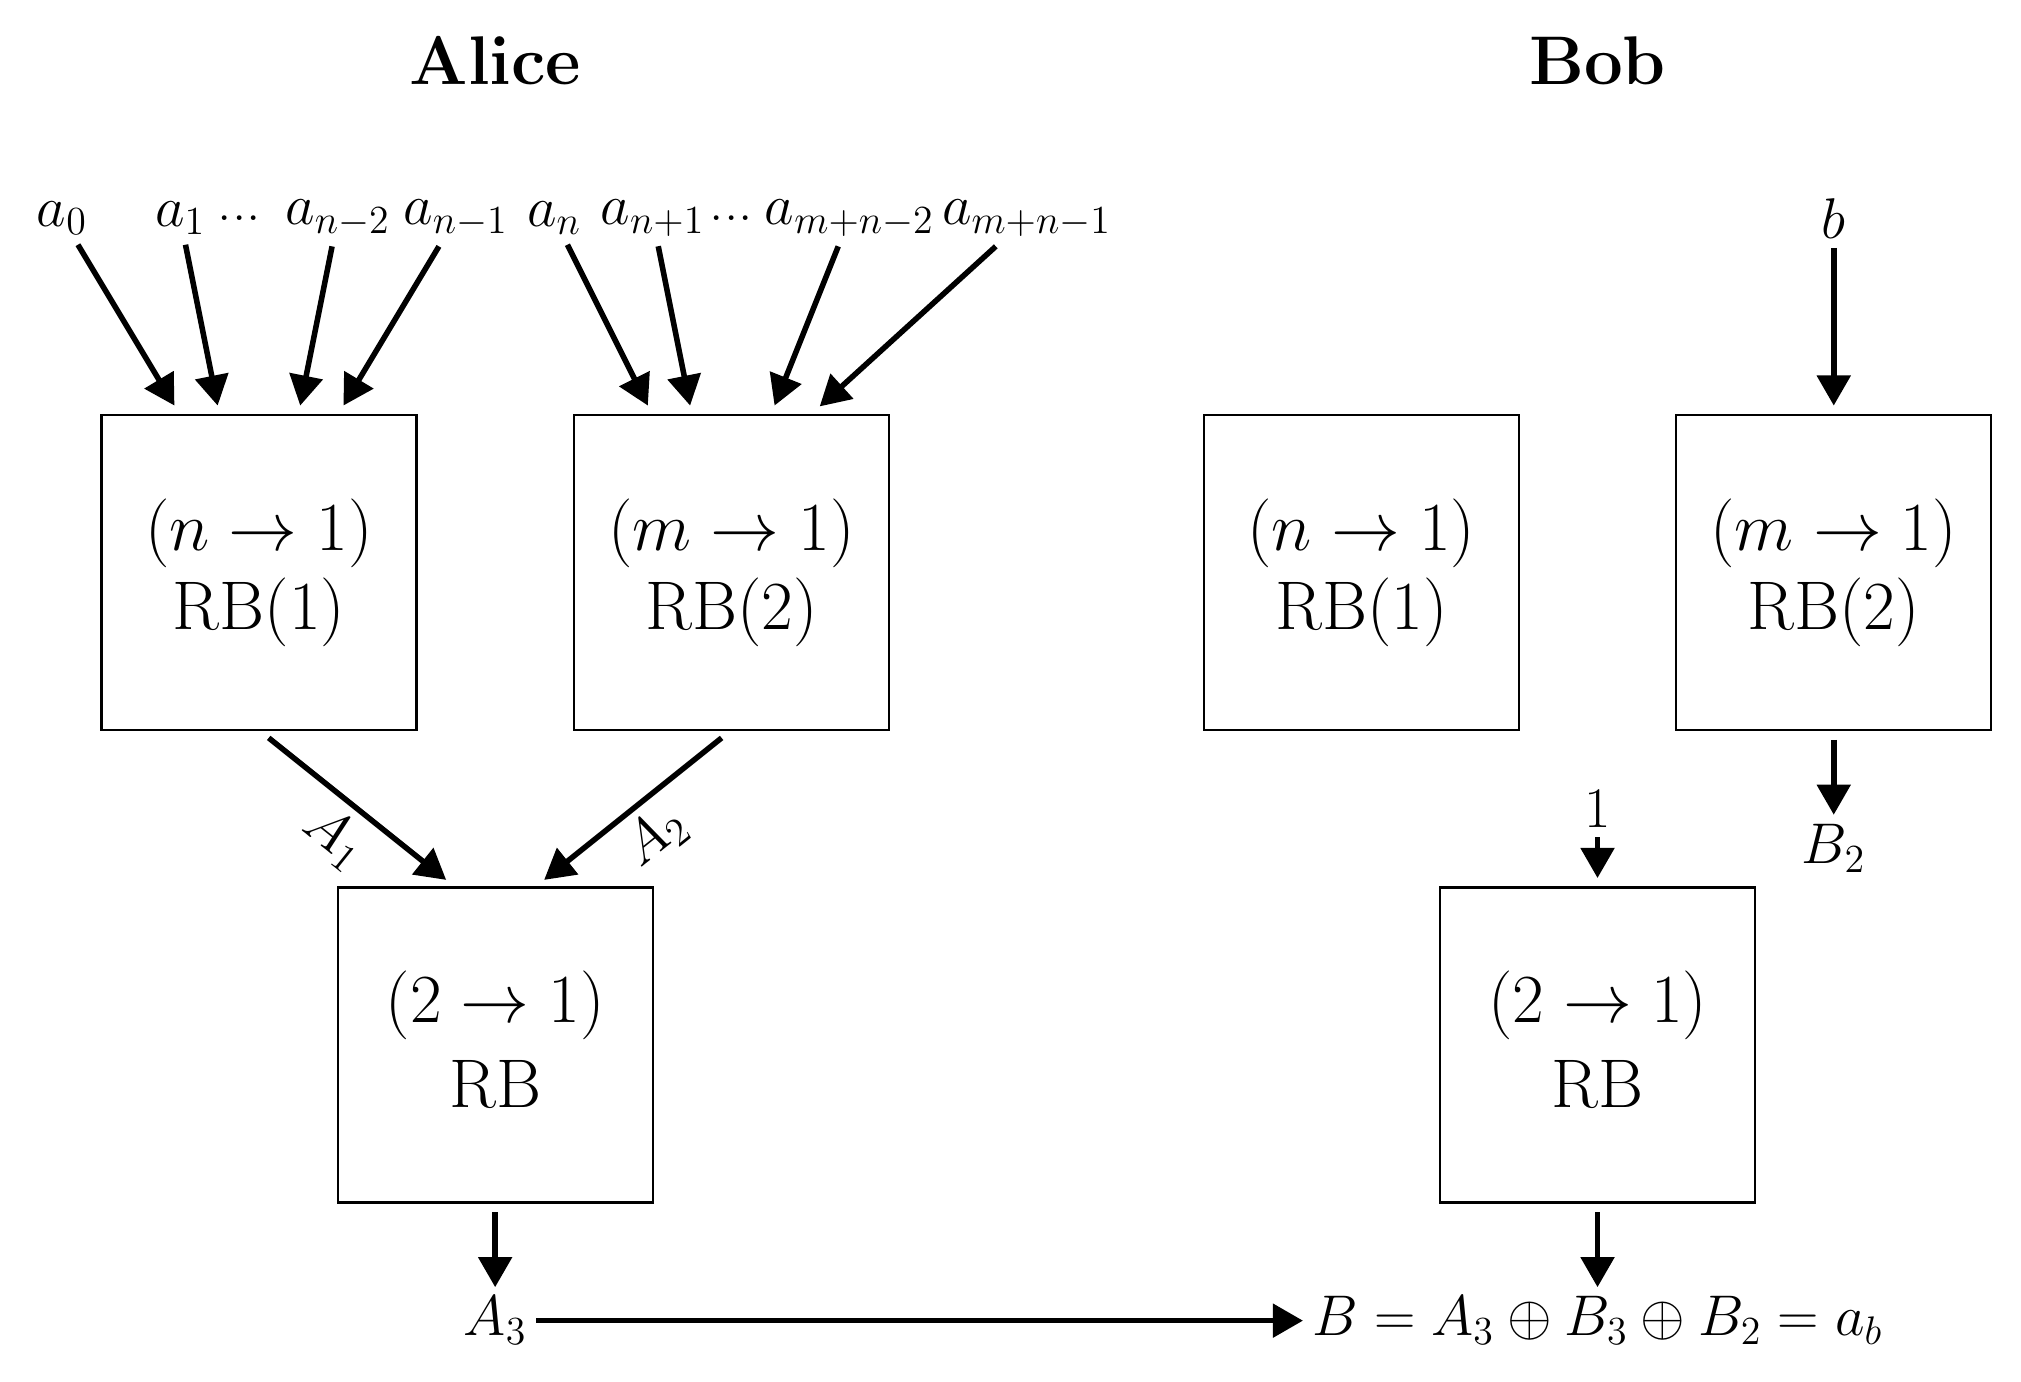
\begin{tikzpicture}
\draw[thick] (-2-6,2+1) rectangle (2-6,-2+1);

\draw[thick]  (-2-12,2+1) rectangle (2-12,-2+1);


\draw[thick]  (-2-9,2-5) rectangle (2-9,-2-5);

\draw[thick] (-2+2,2+1) rectangle (2+2,-2+1);

\draw[thick] (-2+8,2+1) rectangle (2+8,-2+1);

\draw[thick] (-2+5,2-5) rectangle (2+5,-2-5);



\node at (-12,1.5) {\Huge $(n \rightarrow 1)$};
\node at (-6,1.5) {\Huge $(m \rightarrow 1)$};
\node at (2,1.5) {\Huge $(n \rightarrow 1)$};
\node at (8,1.5) {\Huge $(m\rightarrow 1)$};
\node at (5,-4.5) {\Huge $(2\rightarrow 1)$};
\node at (-9,-4.5) {\Huge $(2 \rightarrow 1)$};
\node at (-12,0.5) {\Huge RB(1)};
\node at (-6,0.5) {\Huge RB(2)};
\node at (2,0.5) {\Huge RB(1)};
\node at (8,0.5) {\Huge RB(2)};
\node at (5,-5.5) {\Huge RB};
\node at (-9,-5.5) {\Huge RB};
\node at (-9,7.5) {\Huge \bf Alice};
\node at (5,7.5) {\Huge \bf Bob};
\node (v10) at (-13,3) {};
\node (v12) at (-12.5,3) {};
\node (v14) at (-11.5,3) {};
\node (v16) at (-11,3) {};
\node (v18) at (-7,3) {};
\node (v20) at (-6.5,3) {};
\node (v22) at (-5.5,3) {};
\node (v25) at (-5,3) {};

\node (v2) at (-9.5,-3) {};
\node (v4) at (-8.5,-3) {};

\node (v1) at (-12,-1) {};
\node (v3) at (-6,-1) {};

\draw [-triangle 60,line width=2pt] (v1) edge node[sloped, below] {\huge $A_1$} (v2);
\draw [-triangle 60,line width=2pt] (v3) edge node[sloped,below] {\huge $A_2$} (v4);


\node (v5) at (-9,-7) {};
\node (v6) at (-9,-8.5) {\huge $A_3$};

\draw [-triangle 60,line width=2pt] (v5) edge (v6);
\node (v7) at (5,-7) {};
\node (v8) at (5,-8.5) {\huge $B=A_3 \oplus B_3 \oplus B_2=a_b$};
\draw [-triangle 60,line width=2pt] (v7) edge (v8);
\draw [-triangle 60,line width=2pt] (v6) edge (v8);
\node (v9) at (-14.5,5.5) {\huge $a_0$};
\node (v11) at (-13,5.5) {\huge $a_1$ };
\node (v13) at (-11,5.5) {\huge $a_{n-2}$};
\node (v15) at (-9.5,5.5) {\huge $a_{n-1}$};
\node at (-12.25,5.5) {\huge ...};
\draw [-triangle 60,line width=2pt] (v9) edge (v10);
\draw [-triangle 60,line width=2pt] (v11) edge (v12);
\draw [-triangle 60,line width=2pt] (v13) edge (v14);
\draw [-triangle 60,line width=2pt] (v15) edge (v16);
\node (v17) at (-8.25,5.5) {\huge $a_{n}$};
\node (v19) at (-7,5.5) {\huge $a_{n+1}$};
\node (v21) at (-6,5.5) {\huge ...};
\node (v23) at (-4.5,5.5) {\huge $a_{m+n-2}$};
\node (v24) at (-2.25,5.5) {\huge $a_{m+n-1}$};
\draw [-triangle 60,line width=2pt] (v17) edge (v18);
\draw [-triangle 60,line width=2pt] (v19) edge (v20);
\draw [-triangle 60,line width=2pt] (v23) edge (v22);
\draw [-triangle 60,line width=2pt] (v24) edge (v25);
\node (v26) at (8,5.5) {\huge $b$};
\node (v27) at (8,3) {};
\node (v28) at (8,-1) {};
\node (v29) at (8,-2.5) {\huge $B_2$};
\node (v30) at (5,-2) {\huge $1$};
\node (v31) at (5,-3) {};
\draw [-triangle 60,line width=2pt] (v26) edge (v27);
\draw [-triangle 60,line width=2pt] (v28) edge (v29);
\draw [-triangle 60,line width=2pt] (v30) edge (v31);
\end{tikzpicture}
